
\section{IPOL web interface}

current version is 3.0.

\subsection{Introduction}
The IPOL demo Web interface has been developed with HTML5, CSS3 and Jquery. 
This web page is responsible for letting the users execute demos using either blobs 
from the demo or blobs uploaded by the user.
These are the main points describing the web interface:
\begin{itemize}
  \item Modules.
  \item Flow diagram.
  \item External modules.
  \item Async calls.
  \item Data types.
\end{itemize}



\section{Modules}
This section will try to explain the different modules existing in the demo app. All of these
 modules are divided across the javascript files of the application.
\begin{itemize}
	\item Inputs.
	\item Upload.
	\item Editor.
	\item Parameters.
	\item Run.
	\item Results.
	\item Helpers.
\end{itemize}

\subsection{Inputs}
This module will do everything related to the demo blobs. As it is the starting point of the 
application it will also make the Async calls needed to obtaing data from the demo using id from the URL, like demoinfo 
and blobs back-end modules. These two calls will obtaing the information necesary to execute the demo, letting the 
user choose along the way the input blobs, edit these blobs and tweak demo execution parameters.
This input module will let the user choose among blobs that the demo provides. These blobs will be either images, video or 
audio blobs primarily. It will display a line of blobs or sets of blobs to choose from.


\subsection{Upload}
If the user wants to use their own blobs for the demo this module will let you upload them. Every demo has predefined 
upload slots each with their own characteristics. The user will be able to upload a minimum required number of uploads.
This module will listen for events en every upload slot and get the file information in order to upload them when the run 
button is pressed.

\subsection{Editor}
This module will load after the user selects a set of blobs to run the demo with or when the user uploads their corresponding 
blobs. It will load a view of the chosen blobs where there will be a zoom and crop functions when the sets have 
one blob per set. When the sets have more than one blob per set, the user will also be able a compare button but not a crop 
option.

\subsection{Parameters}
This module will print itself after the user chooses the blobs to use with the demo. It will print itself after the editor and will 
contain as many parameters as the DDL specifies. Parameters have their own specification as well as different types.
The user will be able to tweak them between it's value limitations defined in the DDL.

\subsection{Run}
This module will compile all the blobs and requirements needed to run the demo and will send this information to the demorunner module, then it will wait until there is a response and print the results.

\subsection{Results}
This module will print the results the demorunner gives back letting the user compare the input and results.

\subsection{Helpers}
This module act as an interface for common utility methods like read and write to sessionStorage, make http requests and 
read the origin of the chosen blobs for the demo.

\includegraphics[width=\textwidth]{images/client_server_interaction}

%--------------------------------------------------------------------------------

\section{Flow diagram}
The first thing the application will do when loaded is look for an id which represents
the demo id to be represented. This id will be a parameter inside the URL.
At the same time the main file, demo.js will load the different html files into the DOM
as they have been divided into various files to improve mantainability and coupling.

After all this is loaded, the app will continue adding the main section to the DOM,
 containg in this case the blobs viewer and the blobs upload dialog. At the same time, the 
 the information regarding the current demo, responses from blobs and demoInfo modules 
 will be saved at sessionStorage.
 
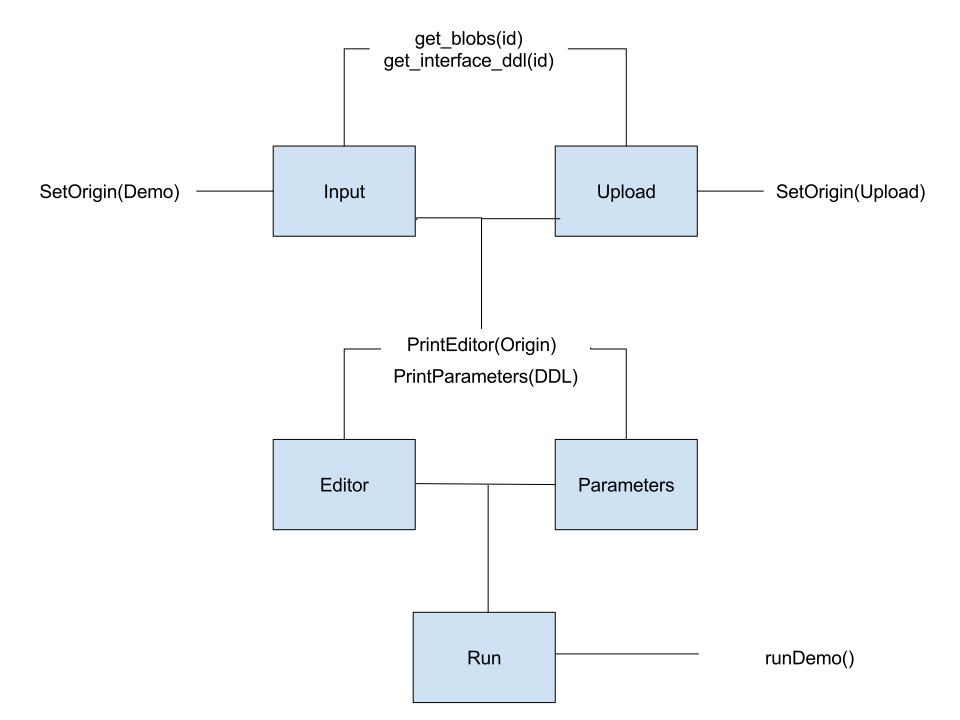
\includegraphics[width=\textwidth]{images/flow}

As the diagram shows, either input or upload modules will pass information to the following modules. Each will set a variable in sessionStorage 
that will indicate if the user has chosen to upload blobs for the demo or a default blob from the list. 

After the user chooses a blob, the editor and parameter modules will load independently and wait for changes. Editor will allow to either 
zoom, crop and compare blobs when possible, as well as do inpainting operations when the demo requires it. The parameters will allow  
tweaking according to ddl specification. Parameter values will be stored in a variable for refreshing feature purpose as the ddl states. 

After the user hits the run button an http post will be executed to run the demo and send the necessary information and wait for a response. 
When the response is obtained it will either print the results interface or the error message.

%--------------------------------------------------------------------------------

\subsection{External modules}

The IPOL demo Web interface uses external libraries, or modules, to add functionalities for the users.
Currently it uses:

\begin{itemize}
\item Cropper.js: Cropper.js it is a simple image cropping JQuery plugin. It is used in the editor panel with the image blobs.
\end{itemize}

%--------------------------------------------------------------------------------

\subsection{Async calls}
The IPOL demo Web interface uses Async calls to get the necessary information from the IPOL server and use it.
This web page shows some information when the async call ends, depends on which one is called.
The current version uses Async calls for:
\begin{itemize}
\item Get the demo ddl: Used to show the inputs description and the upload modal in the Inputs panel, also uses this information to show the parameters.
\item Get blobs: Used to show the blobs in the inputs panel.
\item Run demo: It will send all parameters needed to run the demo and will responde with either the results of the demo or an error response.
\end{itemize}

%--------------------------------------------------------------------------------

\subsection{Data types}
The IPOL platform supports mainly images, but recent updates include audio and video files to use in demos. The new web interface 
allows to choose a set with any combination of images, audio and video. Depending on the data types and sets length options will vary. 
If a set contains multiple images, the user will be able to compare and make zoom using any image on the set. If the user chooses a set with only 
one image blob, options will depend on DDL limitations and will include zoom and crop features, as well as inprinting editing.

In case of uploading an audio or video file, it wont have a visual representation at the moment, only videos and audio files in the default set from the demo will have a visual representation.